% FortySecondsCV LaTeX template
% Copyright © 2019-2022 René Wirnata <rene.wirnata@pandascience.net>
% Licensed under the 3-Clause BSD License. See LICENSE file for details.
%
% Please visit https://github.com/PandaScience/FortySecondsCV for the most
% recent version! For bugs or feature requests, please open a new issue on
% github.
%
% Contributors:
% https://github.com/PandaScience/FortySecondsCV/graphs/contributors
%
% Attributions
% ------------
% * fortysecondscv is based on the twentysecondcv class by Carmine Spagnuolo
%   (cspagnuolo@unisa.it), released under the MIT license and available under
%   https://github.com/spagnuolocarmine/TwentySecondsCurriculumVitae-LaTex
% * further attributions are indicated immediately before corresponding code


%-------------------------------------------------------------------------------
%                             ADDITIONAL PACKAGES
%-------------------------------------------------------------------------------
\documentclass[
	a4paper,
	9pt,
	sidesectionsize=Large,
	itemtextcolor=black!75,
	sidebarwidth=0.36\paperwidth,
	topbottommargin=0.025\paperheight,
	leftrightmargin=15pt,
	profilepicsize=4.2cm,
	profilepicborderwidth=2pt,
	profilepicstyle=profilecircle,
	profilepiczoom=1.05,
	datecolwidth=0.2\textwidth,
]{fortysecondscv}

% fine tune line spacing
\usepackage{setspace}
\setstretch{1.05}

% improve word spacing and hyphenation
\usepackage{microtype}
\usepackage{ragged2e}

% uncomment in case you don't want any hyphenation
% \usepackage[none]{hyphenat}

% take care of proper font encoding
\ifxetexorluatex
	\usepackage{fontspec}
	\defaultfontfeatures{Ligatures=TeX}
	% \newfontfamily\headingfont[Path=fonts/]{segoeuib.ttf} % use local font
\else
	\usepackage[utf8]{inputenc}
	\usepackage[T1]{fontenc}
\fi

% use a sans serif font as default
\usepackage[sfdefault]{ClearSans}

% enable mathematical syntax for some symbols like \varnothing
\usepackage{amssymb}

% redefine icon commands for consistent sizing and spacing
\renewcommand*{\socialicon}[1]{%
	\makebox[1.2em][l]{\textcolor{iconcolor}{#1}}%
}
\renewcommand*{\circleicon}[1]{%
	\makebox[1.2em][l]{\textcolor{iconcolor}{#1}}%
}

% bubble diagram configuration
\usepackage{smartdiagram}
\smartdiagramset{
	% default font size is \large, so adjust to harmonize with sidebar layout
	bubble center node font = \footnotesize,
	bubble node font = \scriptsize,
	% default: 4cm/2.5cm; make minimum diameter relative to sidebar size
	bubble center node size = 0.35\sidebartextwidth,
	bubble node size = 0.22\sidebartextwidth,
	distance center/other bubbles = 1.3em,
	% set center bubble color
	bubble center node color = maincolor!70,
	% define the list of colors usable in the diagram
	set color list = {maincolor!10, maincolor!40,
	maincolor!20, maincolor!60, maincolor!35},
	% sets the opacity at which the bubbles are shown
	bubble fill opacity = 0.8,
}

\newcommand{\intro}[3]{%
	{\Huge\color{sectioncolor}{#1}}\par%
	\setlength{\parskip}{1.8ex}
	{\Large\color{black!80}{#2}}\par%
	\setlength{\parskip}{0.8ex}
	\parbox[b]{\linewidth}{\textcolor{itemtextcolor}{#3}}
}

%-------------------------------------------------------------------------------
%                            PERSONAL INFORMATION
%-------------------------------------------------------------------------------
%% mandatory information
% your name
\newcommand{\name}{\textbf{Dr. Vanda} Farsad}
\cvname{\name}
% job title/career
\newcommand{\jobtitle}{Backend-Entwicklerin} 
\cvjobtitle{\jobtitle}

%% optional information
% profile picture
\cvprofilepic{pics/vanda.pdf}
% logo picture
% \cvlogopic{pics/logo_txt.png}

% NOTE: ordering in sidebar will mimic the following order
% date of birth
\cvbirthday{August 1, 1981}
% short address/location, use \newline if more than 1 line is required
\cvaddress{Am Inselpark 9, 21109 Hamburg}
% phone number
\cvphone{+49 172 289 08 37}
% \cvsite{www.initial-commit.com}
\cvmail{v.farsad@initial-commit.com}
% \cvsite{www.initial-commit.com}

%-------------------------------------------------------------------------------
%                              SIDEBAR 1st PAGE
%-------------------------------------------------------------------------------
% add more profile sections to sidebar on first page
\addtofrontsidebar{
	% include gosquare national flags from https://github.com/gosquared/flags;
	% naming according to ISO 3166-1 alpha-2 country codes
	\graphicspath{{pics/gosquared-flags/flags/flags-iso/shiny/64}}


	% \sidesection{About me}
	% \aboutme{
	% 	Hello there! With expertise in Python and experience in both DevOps and frontend technologies, 
	% 	I'm eager to assist you with the design, creation, or optimization of your web application.}

	% social network accounts incl. proper hyperlinks
	\sidesection{Links}
		\begin{icontable}[1.6]{1.2em}{0.5em}
			\social{\faGlobe}
				{https://www.initial-commit.com}
				{Webseite}
			\social{\faLinkedin}
			{https://www.linkedin.com/in/vanda-farsad-4b98321a5/}
			{LinkedIn}
			\social{\faGithub}
			{https://github.com/VandaFarsad}
			{Github}
		\end{icontable}
		
	\sidesection{Stack}
	\begin{figure}\centering
		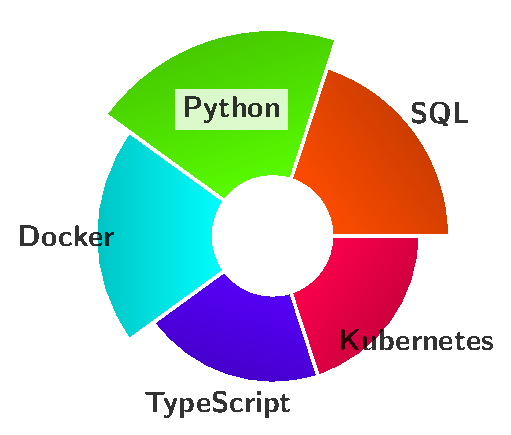
\includegraphics[scale=0.72]{pics/diagrams/stack.pdf}
	\end{figure}

	\sidesection{Frameworks}
	\pointskill{\faPython}{Django}{5}
	\pointskill{\faReact}{Next.js}{3}
	\pointskill{\faReact}{React}{2}
	\pointskill{\faPython}{Flask}{2}

	\sidesection{Sprachen}
	\pointskill{\flag{DE.png}}{Deutsch}{5}
	\pointskill{\flag{GB.png}}{Englisch}{3}
	\pointskill{\flag{IR.png}}{Persisch}{2}

}


%-------------------------------------------------------------------------------
%                              SIDEBAR 2nd PAGE
%-------------------------------------------------------------------------------
\definecolor{pastelgreen}{HTML}{D7ECD9}
\definecolor{pastelpurple}{HTML}{D5D6EA}
\definecolor{pastelorange}{HTML}{F5D5CB}
\definecolor{pastelyellow}{HTML}{F6F6EB}

\addtobacksidebar{
	\sidesection{About Me}
	\aboutme{
		The giant panda is a terrestrial animal and primarily spends its life
		roaming and feeding in the bamboo forests of the Qinling Mountains and in
		the hilly province of Sichuan.
	}

	\sidesection{Diagrams}
	\begin{sidebarminipage}
		\chartlabel[pastelgreen]{Bubble}
		\chartlabel[pastelgreen]{Diagrams}
		\chartlabel[pastelpurple]{with}
		\chartlabel[pastelpurple]{proper}
		\chartlabel[pastelorange]{overflow}
		\chartlabel[pastelorange]{protection}
		\chartlabel[pastelyellow]{for}
		\chartlabel[pastelyellow]{labels}
	\end{sidebarminipage}

	\begin{figure}\centering
		\smartdiagram[bubble diagram]{
			\textcolor{white}{\textbf{Being a}} \\
			\textcolor{white}{\textbf{Panda}}, % center bubble
			\textcolor{black!90}{Eating},
			\textcolor{black!90}{Sleeping},
			\textcolor{black!90}{Rolling},
			\textcolor{black!90}{Playing},
			\textcolor{black!90}{Chilling}
		}
	\end{figure}

	\chartlabel{Wheel Chart}

	\wheelchart{3.7em}{2em}{%
	20/3em/maincolor!50/Chill,
	15/3em/maincolor!15/Play,
	30/4em/maincolor!40/Sleep,
	20/3em/maincolor!20/Eat
	}

	\sidesection{Barskills}
	\barskill[1ex]{\faSkyatlas}{Wearing asian rice hats}{60}
	\barskill[2ex]{\faImage}{Playing Chess}{30}
	\barskill[3ex]{\faMusic}{Playing the bamboo flute}{50}

	\sidesection{Memberships}
	\begin{memberships}
		\membership[4em]{pics/logo.png}{PandaScience.net}
		\membership[4em]{pics/logo.png}{Some longer text spanning over more than
			only one line}
	\end{memberships}
}


%-------------------------------------------------------------------------------
%                         TABLE ENTRIES RIGHT COLUMN
%-------------------------------------------------------------------------------
\begin{document}

\makefrontsidebar

\newgeometry{left=3.1in, right=0.3in, top=0.75in, bottom=0.5in}

\intro{\name}{\jobtitle}{
	Hallo! Ich bringe Erfahrung in Python, moderner Frontend-Entwicklung und ein solides Verständnis von DevOps mit. 
	Was mir am wichtigsten ist: Code zu schreiben, der nicht nur funktioniert, sondern auch wartbar, testbar und 
	nachhaltig ist.
	\\\\
	Ob Backend-Architektur oder Frontend-UX -- ich arbeite gerne an Projekten, die Effizienz, Qualität und 
	Innovation verbinden. Am meisten Freude macht mir, Ideen im Team zur Realität zu machen und Lösungen zu 
	schaffen, die echten Mehrwert liefern.
}

\cvsection{Berufserfahrung}
\begin{cvtable}[3]
	\cvitem{seit 2020}{Freiberufliche Fullstack-Entwickler}{Orendt Studios}{Entwicklung, Test und Wartung von Django-basierten
		Webanwendungen, CI/CD-Pipelines und Frontend-Frameworks.
		Verwaltung des kompletten Entwicklungslebenszyklus von Projekten, von der strategischen Planung bis zur 
		erfolgreichen Implementierung und Übernahme der Verantwortung für Zeitpläne.\\\\
		Backend-Technologien: Python (Django, Flask)\\
		Frontend-Technologien: Typescript (Next.js, React)\\
		CI/CD-Tools: Docker, Kubernetes, Gitlab, PostgreSQL}
	\cvitem{2019 -- 2019}{Senior Consultant Biostatistik}{Ecker+Ecker}{
		Zusätzlich Projektmanagement.}
	\cvitem{2017 -- 2019}{Consultant Biostatistik}{Ecker+Ecker}{
		Entwicklung von Python-Software für verschiedene Anwendungen, Durchführung von Datenanalysen mit Python und R, 
		Bewertung klinischer Studien, statistische Beratung für Kunden und Teammitglieder sowie Durchführung von 
		Statistik-Schulungen.
	}
	\cvitem{2008 -- 2010}{Wissenschaftlicher Mitarbeiter}{Fraunhofer-Institut LBF}{Durchführung von Methodenimplementierungen
		mit Matlab/Simulink und numerische Simulationen für umfassende Analysen.}
\end{cvtable}


\cvsection{Ausbildung}

\begin{cvtable}[1.5]
	\cvitem{2014 -- 2017}{Promotion $\bullet$ Mathematik (\normalfont{cum laude})}{Universit\"at Hamburg}
	{Dissertation: \emph{The symplectic fermion ribbon quasi-Hopf algebra and the $SL(2,\mathbb{Z})$-action on its centre.}
		\footnote{\href{https://doi.org/10.1016/j.jalgebra.2018.12.012}{
				Journal of Algebra. 522. 10.1016/j.jalgebra.2018.12.012}, 2017.}
		\footnote{\href{https://doi.org/10.1016/j.aim.2022.108247}{
				Advances in Mathematics. 400. 10.1016/j.aim.2022.108247}, 2022.}
	}
	\cvitem{2009 -- 2013}{Master of Science $\bullet$ Mathematik ($\varnothing\, 1,5$)}{TU Darmstadt}
	{Schwerpunkt: Geometrie, Kernphysik und Operatoralgebra}
	\cvitem{2005 -- 209}{Diplom $\bullet$ Ang. Mathematik ($\varnothing\, 1,3$)}{Hochschule Darmstadt}
	{Schwerpunkt: Numerische Mathematik und Informatik (C\texttt{++})}
\end{cvtable}

% \cvsection{Publications}
% \begin{cvtable}
% 	\cvpubitem{Cooking: 100 recipes for lazy Pandas}{Me and My Panda Friends}
% 	{Panda's Culinary World}{2010}
% 	\cvpubitem{Pandastasia}{Still Me}{Bamboo Books Assoc.}{2005}
% \end{cvtable}

% \cvsection{Awards}
% \begin{cvtable}
% 	\cvitem{2010 -- now}{Panda of the Year}{Panda World Forum}{}
% 	\cvitem{2005 -- now}{Face of World Wide Fund for Nature}{WWF}{}
% 	\cvitem{2000}{Winner of Bamboo Sprouts Eating Contest}{Bamboo Society}{}
% \end{cvtable}


% \cvsection{Extra-Curricular Activities}
% \begin{cvtable}
% 	\cvitemshort{Relaxing}{Master the fine art of relaxing everywhere}
% 	\cvitemshort{Music}{Playing the bamboo flute in the 1st Panda Orchestra}
% 	\cvitemshort{Education}{Teaching young pandas to be more panda-like}
% \end{cvtable}


% \newpage
% \makebacksidebar
% % \newgeometry{
% % 	top=\topbottommargin,
% % 	bottom=\topbottommargin,
% % 	right=\leftrightmargin,
% % 	left=\leftrightmargin
% % }

% \cvsection{section}
% \cvsubsection{Subsection}
% \begin{cvtable}
% 	\cvitem{<dates>}{<cv-item title>}{<location>}{<optional: description>}
% \end{cvtable}

% \cvsection{cvitem}
% \cvsubsection{Multi-line with longer description}
% \begin{cvtable}
% 	\cvitem{date}{Description}{location}{Some longer and more detailed
% 		description, that takes two lines of space instead of only one.}
% 	\cvitem{date}{Description}{location}{Some longer and more detailed
% 		description, that takes two lines of space instead of only one.}
% 	\cvitem{date}{Description}{location}{Some longer and more detailed
% 		description, that takes two lines of space instead of only one.}
% \end{cvtable}

% \cvsubsection{One-line without description}
% \begin{cvtable}
% 	\cvitem{Award}{One-line description}{Sponsor}{}
% 	\cvitem{Award}{One-line description}{Sponsor}{}
% 	\cvitem{Award}{One-line description}{Sponsor}{}
% \end{cvtable}

% \cvsection{cvitemshort}
% \cvsubsection{One-line}
% \begin{cvtable}
% 	\cvitemshort{Key}{Some further description}
% 	\cvitemshort{Key}{Some further description}
% 	\cvitemshort{Key}{Some further description}
% \end{cvtable}

% \cvsubsection{Multi-line with longer description}
% \begin{cvtable}
% 	\cvitemshort{Key}{Some further description. Can fill even more than
% 		only one single line while still keeping the correct indendation level.}
% 	\cvitemshort{Key}{Some further description. Can fill even more than
% 		only one single line while still keeping the correct indendation level.}
% 	\cvitemshort{Key}{Some further description. Can fill even more than
% 		only one single line while still keeping the correct indendation level.}
% \end{cvtable}

% \cvsection{cvpubitem}
% \begin{cvtable}
% 	\cvpubitem{Publication title}{Authors}{Journal}{Year}
% 	\cvpubitem{Publication title}{Authors}{Journal}{Year}
% 	\cvpubitem{Publication title that is spanning over multiple lines and still
% 		does not look too bad}{Authors}{Journal}{Year}
% \end{cvtable}

% \cvsignature

\end{document}
